\chapter{Metodologia} \label{cap:metodologia}

Neste capítulo os detalhes envolvidos na geração das imagens de CAPTCHAs são expostos. Em seguida, definimos as grandezas de interesse que nos permitem acessar a qualidade dos modelos treinados. Por fim, as etapas de treino e validação são formalizadas.


\section{Geração dos CAPTCHAs}

Todos os exemplos foram gerados utilizando a biblioteca SimpleCaptcha\cite{simplecaptcha}. Ao total, foram gerados $30000$ pares imagem-token.
As sequências de texto possuem comprimento fixo em $5$ e os caracteres foram sorteados de forma independente a partir do alfabeto ordenado $\Sigma = \{0123456789abcdefghijklmnopqrstuvwxyz\}$ de $36$ símbolos. Dentre os efeitos escolhidos para as imagens, enfatizamos as variações nas cores de fundo, desenho de grades, adição de linhas aleatórias e deformação em explosão, que são técnicas efetivas para construir desafios fáceis para humanos e difíceis para computadores, de acordo com estudo conduzido por \cite{lectures2005HIP}. Uma pequena amostra dos pares imagen-token gerados pode ser vista na Fig.\ref{imgcaptchas}. 

\begin{figure}[ht]
	\begin{subfigure}{.5\textwidth}
		\centering
		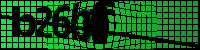
\includegraphics[width=.9\linewidth]{figuras/7103_b26bf.png}
		\caption{b26bf}
	\end{subfigure}
	\begin{subfigure}{.5\textwidth}
		\centering
		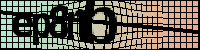
\includegraphics[width=.9\linewidth]{figuras/9456_ep8nb.png}
		\caption{ep8nb}
	\end{subfigure}%
	\vspace{.05\linewidth}
	
	\begin{subfigure}{.5\textwidth}
		\centering
		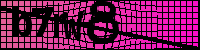
\includegraphics[width=.9\linewidth]{figuras/21856_b7rw8.png}
		\caption{b7rw8}
	\end{subfigure}
	\begin{subfigure}{.5\textwidth}
		\centering
		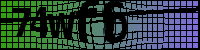
\includegraphics[width=.9\linewidth]{figuras/19816_74wf6.png}
		\caption{74wf6}
	\end{subfigure}%
	\vspace{.05\linewidth}
	
	\begin{subfigure}{.5\textwidth}
		\centering
		
\includegraphics[width=.9\linewidth]{figuras/12248_dnyny.png}
		\caption{dnyny}
	\end{subfigure}
	\begin{subfigure}{.5\textwidth}
		\centering
		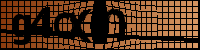
\includegraphics[width=.9\linewidth]{figuras/8873_g4cxh.png}
		\caption{g4cxh}
	\end{subfigure}%
	\vspace{.05\linewidth}
	\caption{Exemplos de CAPTCHAs gerados e seus respectivos tokens.}
	\label{imgcaptchas}
\end{figure}

Considere $D = {(x, y)}$ o conjunto formado por todos os pares de imagem-token gerados. Durante o treino, cada exemplo de entrada é formado por um tensor imagem $x$ e uma matriz $y$ representando o token correto $u$, de dimensões $(200, 50, 3)$ e $(5, 36)$, respectivamente. Ao realizar uma predição, apenas a entrada $x$ é fornecida à rede. Cada $x_{ijk} \in \Re[0,1]$ representa a intensidade do pixel localizado na posição $(i,j)$ e canal $k$, enquanto $y_{ij} \in \Re[0,1]$ foi codificado utilizando-se a técnica \textit{one-hot encoding}, onde $i$ representa a posição na sequência $u$ e $j$ o índice no vocabulário do caractere nessa posição, de modo que 
\begin{equation}\label{eq:yasprob}
   y_{ij}= 
	\begin{cases}
		1,	& \text{se } u_i = \Sigma_j\\
		0,  & \text{caso contrário,}
	\end{cases}
\end{equation}
ou, de forma mais compacta, $y_{ij} = \delta_{u_i,\Sigma_j}$, onde $\delta_{m,n}$ é o delta de Kronecker. Essa codificação nos permite interpretar $y$ como sendo uma distribuição de probabilidade. Se imaginarmos $z$ como uma variável aleatória descrevendo a i-\textit{ésima} entrada na sequência, e $p_i(z|x)$ como a probabilidade de na posição $i$ da sequência termos o caractere $z$ dada a imagem $x$, para os exemplos gerados, o conhecimento da imagem define automaticamente qual o caractere em cada posição com $100\%$ de certeza, ou seja, se $c$ é o caractere de fato na sequência ($c = u_i$), teremos $p_i(z = c|x) = p_i(z = u_i|x) = 1$ e, caso contrário, $p_i(z \neq c|x) = p_i(z \neq u_i|x) = 0$. Ou, utilizando o delta de Kronecker, $p_i(z|x) = \delta_{z,u_i}$. Definindo $ord(c)$ como o índice do caractere $c$ no alfabeto $\Sigma$ (isto é, $c = \Sigma_{ord{(c)}}$), da equação \ref{eq:yasprob} vem que, $p_i(z|x) = \delta_{z,u_i} = \delta_{u_i, z} = \delta_{u_i, \Sigma_{ord(z)}} = \delta_{u_i,\Sigma_j} = y_{ij}$.

A saída da rede neural é a matriz $\hat{y} = f^{\Theta}(x)$, a distribuição de probabilidade inferida pela rede. O caractere predito pela rede na posição $i$ é dado pelo caractere mais provável nessa distribuição nesta posição, isto é, $\Sigma_{\argmax_j \hat{y}_{ij}}$, sendo o token predito formado pelos caracteres mais prováveis em cada posição. Nosso objetivo é encontrar $\hat{y}$ como uma aproximação para $y$.

Para a preparação da base, o $D$ foi reordenando de forma aleatória e separado em dois subconjuntos: o conjunto de treino, $D_{tr}$, com $\frac{2}{3}$ do total de pares, e o conjunto de validação, $D_{val}$, com os demais exemplos. Devido à natureza combinatória do espaço de imagens possíveis ($36^5$ tokens $\times$ $255^3$ cores de fundo $\times$ espaço de todas as pertubações possíveis), $D$ é muito menor do que o conjunto de todas as possíveis composições imagem-token e, supondo que seus elementos tenham sido construídos ao acaso, é virtualmente improvável que existam exemplos repetidos nesse conjunto.

\section{Treino e Validação}

Uma época de aprendizado consiste em duas etapas: treino e validação. Durante o treino, um subconjunto $D_{batch} \subset D_{tr}$ é sorteado ao acaso. Os parâmetros da rede são atualizados utilizando o algoritmo adaptativo Adam com os parâmetros sugeridos em\cite{adam_op} ($\beta_1 = 0.9$, $\beta_2 = 0.999$ e $\epsilon = 10^{-8}$) e taxa de aprendizado $l_r$ de forma a minimizar o erro nesse subconjunto. A subetapa de treino (treino dentro de uma época) se encerra após $|D_{tr}|/|D_{batch}|$ atualizações. Na etapa de validação, as grandezas de interesse são calculadas para $D_{tr}$ e $D_{val}$ e salvas para posterior análise. Em todos os experimentos fixamos $|D_{batch}| = 10$ exemplos.

As redes foram inicializadas segundo a heurística proposta em \cite{HeZR015relu} e as épocas de aprendizado se sucedem até que o critério de parada ser alcançado. Escolhemos como critério de parada uma heurística semelhante às definidas por \cite{lutz_early_stop}. A dinâmica de aprendizado leva no mínimo $T^{min}$ e no máximo $T^{max}$ épocas. Após a etapa de validação o aprendizado é interrompido prematuramente se um dos dois critérios forem verificados: o custo calculado em $D_{val}$ na época atual ultrapasse em mais de $10\%$ o menor valor de $J^{(D_{val})}$ nas épocas anteriores; o valor de $J^{(D_{tr})}$ atual seja maior do que $97\%$ da média dos cinco últimos custos nesse conjunto. Ou seja, o treinamento é parado prematuramente se for detectado \textit{overfitting} ou se não houver melhora significativa em relação aos últimos valores.

Para selecionar o valor do hiper-parâmetro $l_r$, foram realizados experimentos com diferentes valores fixos de $l_r$ e $T^{max}=10$ épocas para cada arquitetura. A partir dos experimentos, selecionamos manualmente os limites inferior e superior, ($l_r^-$, $l_r^+$), que apresentam o melhor compromisso entre velocidade de aprendizado e estabilidade (vide seção \ref{sec:aprendizado}). Os experimentos posteriores foram realizados com uma taxa de aprendizado segundo a equação:
\begin{equation}
l_r(t) = l_r^+ + (l_r^- - l_r^+) * \frac{t}{T_{max}-1},
\end{equation}
onde $t = 0, 1, 2, \ldots, T_{max}-1$, onde $t$ é a época atual.

Todos os experimentos realizados nesse trabalho foram executados ema máquina com processador Intel\textsuperscript{\textregistered} Core\texttrademark i5-6200U, 8gb de RAM e placa de aceleração gráfica NVIDIA\textsuperscript{\textregistered} 920M com 2 gb de memória, utilizando a biblioteca de código aberto Tensorflow \cite{abadi2016tensorflow}.

\section{Métricas}

No capítulo de fundamentação teórica de redes neurais (capítulo \ref{cap:neurais}), vimos que cada arquitetura é parametrizada $\Theta$. Mais especificamente, cada uma das arquiteturas utilizadas neste trabalho possui como parâmetros um conjuntos de números reais. Assim, definimos o \textbf{tamanho do modelo}, para fins de comparação, como a soma da quantidade de parâmetros de cada camada da arquitetura. Para treinar e avaliar a qualidade dos modelos, consideramos as grandezas definidas à seguir. Em todas as definições, considere $D$ um conjunto de exemplos, $(x,y) \in D$ e $\hat{y} = f^{\Theta}(x)$ a distribuição de probabilidade inferida pelo modelo (eq. \ref{eq:yasprob}). 

Para avaliar o erro cometido pelos classificadores, podemos utilizar a \textbf{entropia cruzada} (no inglês \textit{cross entropy}), que pode ser interpretada como uma medida de divergência entre duas distribuições de probabilidade. Assim, o custo associado ao inferir $\hat{y}$ quando a verdadeira distribuição deveria ser $y$, por caractere, é dado por
\begin{align}
	H_i(y, \hat{y}) &= -\sum_j y_{ij} \log_2{\hat{y}_{ij}} \\
					&= -\sum_j \delta_{u_i, \Sigma_{j}} \log_2{\hat{y}_{ij}} \\
					&= -\log_2{\hat{y}_{i\;ord(u_i)}}
\end{align}
onde utilizamos o fato de $\delta_{u_i, \Sigma_{j}} = 0$ exceto em $j = ord(u_i)$. Em outras palavras, a entropia associada ao classificador da posição $i$ é o logaritmo da probabilidade predita para o caractere correto nessa posição. Definimos o \textbf{custo esperado por caractere} do classificador $i$ em $D$ como 
\begin{equation} \label{lossi} 
	J_i^{(D)} = \frac{1}{|D|} \sum_{(x,y) \in D} H_i(y, \hat{y})
\end{equation}
e \textbf{custo esperado por token} como a média dos erros em cada posição, ou seja:
\begin{equation} \label{loss}
	J^{(D)} = \langle J_i^{(D)} \rangle_{\{i\}} .
\end{equation}
Durante o treino tentaremos minimizar a \ref{lossi} para cada classificador, e o custo total associado aos erros cometidos pelo modelo é calculado pela equação \ref{loss}.

Uma estimativa da probabilidade de acerto por caractere é dada pela \textbf{acurácia de cada classificador}, isto é, o número de acertos do caractere $i$ no conjunto $D$, representado por $N_i$, normalizado pelo tamanho do conjunto $D$: 
\begin{equation}
	\hat{p}_i^{(D)} = acc_i^{(D)} = \frac{N_i}{|D|}.
\end{equation}
Estimamos a probabilidade de acerto do token através da \textbf{acurácia do modelo} pela equação:
\begin{equation} \label{eq:accw}
	\hat{p}_u^{(D)} = \frac{N_u}{|D|},
\end{equation}
onde $N_u$ é o número de tokens preditos corretamente.

Quanto ao tempo da dinâmica de aprendizado, definimos, para cada época $t$, o \textbf{tempo de treino por época}, $\tilde{\tau}$, como sendo o tempo gasto durante a fase de treino nessa época e o \textbf{tempo total de uma época}, $\tau$, com a soma dos tempos gastos com treino e validação. Adicionalmente, definimos o \textbf{tempo de convergência}, $T$, como o tempo decorrido até que o critério de parada tenha sido alcançado.